\subsubsection{UC\theuccount-G - GitLab segnala evento di push a Producer GitLab}
	\begin{figure}[H]
		\centering
		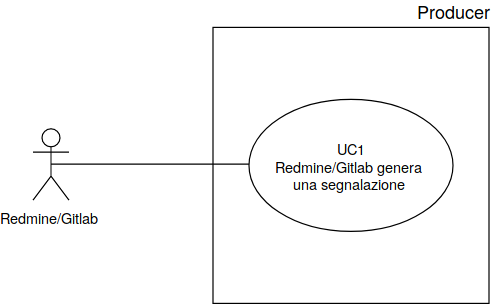
\includegraphics[width=0.7\textwidth]{img/UC1.png}\\
		\caption{UC\theuccount-G - GitLab segnala evento di push a Producer GitLab}
	\end{figure}
	\begin{itemize}
		\item \textbf{Codice}: UC\theuccount-G.
		\item \textbf{Titolo}: GitLab segnala evento di push a Producer GitLab.
		\item \textbf{Attori primari}: GitLab.
		\item \textbf{Descrizione}: l'invio di una segnalazione avviene da parte di GitLab tramite webhook. L'evento di
		push può essere composto da uno o più commit.
		\item \textbf{Precondizione}: Viene effettuato un push su GitLab e segnalato a \progetto.
		\item \textbf{Postcondizione}: il Producer GitLab riceve la segnalazione da GitLab.
		\item \textbf{Scenario principale}: 
		\begin{enumerate}
			\item GitLab procede all'invio della segnalazione di push al Producer GitLab.
		\end{enumerate}
		
	\end{itemize}